\section{Introduction and Game Description}
\subsection{Game Introduction}
\subsubsection{Game rules}
Othello, also called Reversi, is a strategy board game for two players, played 
on an 8*8 uncheckered board. There are sixty-four identical game pieces called 
disks (Black and White). Players take turns placing disks on the board with 
their assigned color facing up. During a play, any disks of the opponent's color 
that are in a straight line and bounded by the disk just placed and another disk 
of the current player's color are turned over to the current player's color.

Only placement of disk that can flip opponent's disk can be considered as a valid placement, otherwise the player cannot put disk at this position. If in a player's turn, no valid placement exists under the situation, it will automatically becomes opponent's turn. If both players don't have a valid placement, the player with more disks win.

\subsubsection{Game objective}
The object of the game is to have the majority of disks turned to display your 
color when the last playable empty square is filled.

\subsection{Design Introduction}

\subsubsection{Join/Create/Speculate a game} There are two ways for a logged-in 
user to join an existing game. He can either 
click the join game button on the index page and type in the existing game name
if he/she knows, or he can enter the game lobby by clicking the 
game lobby button. There are two kinds of game, one is games already started, 
which other users can speculate, the other is games still wait for matching, 
which other users can join to play against others. 

\subsubsection{Speculators and Players authority} We allow anonymous user
(who don't log in) to speculate the game that has started but that user will not
be shown in speaculator list in game page. But one user is only 
be allowed to join or create the game when he/she is logged in. 

\subsubsection{Priority for current players}
When a player creates a new room, the game board is locked, he must wait for an
opponent to join to start the game. After second player enters the room, the board
will be unlocked, first person enter the room will move first. After the game 
start, other users can speculate the game. When one of the players leaves the 
room, the room will still exist, while when both players left the room, the 
room will be deleted and all the speculators will receive an alert and be 
redirected to index page . That's why we call the design choice priority for 
players, as they are the key roles of the game.

\section{UI Design}
There are four main pages in our game.
\subsection{Index Page}
Index page contains the entry to log in, create game and enter game lobby.
\begin{itemize}
\item When click log in, the app will redirect user to log-in page.
\item When click join game button, user can create a new game or join an 
existing game by entering the game name. When hit enter, the app will redirect
user to game page.
\item When click game lobby button, the app will redirect user to lobby page.
\end{itemize}
\begin{figure}[!htb]

\includegraphics[height=2.0in, width=3.3in]{index.png}
\caption{\texttt{Index Page}}
\end{figure}
\begin{figure}[!htb]
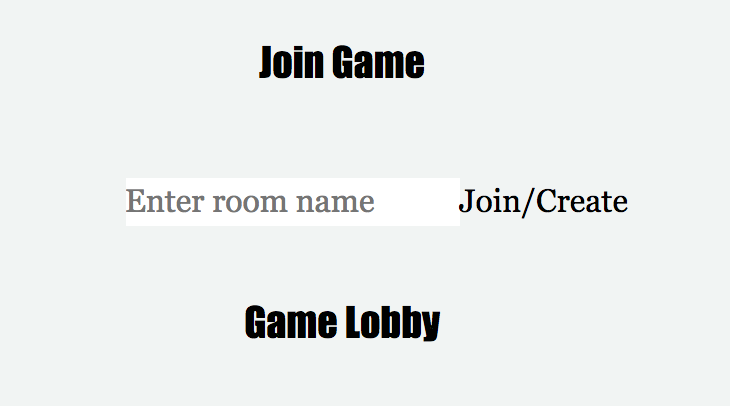
\includegraphics[height=2.0in, width=3.3in]{index2.png}
\caption{\texttt{Join Game Button}}
\end{figure}

\subsection{Log in Page}
Log in part is very basic. User can just enter the name without password to 
log in.
\begin{figure}[!htb]
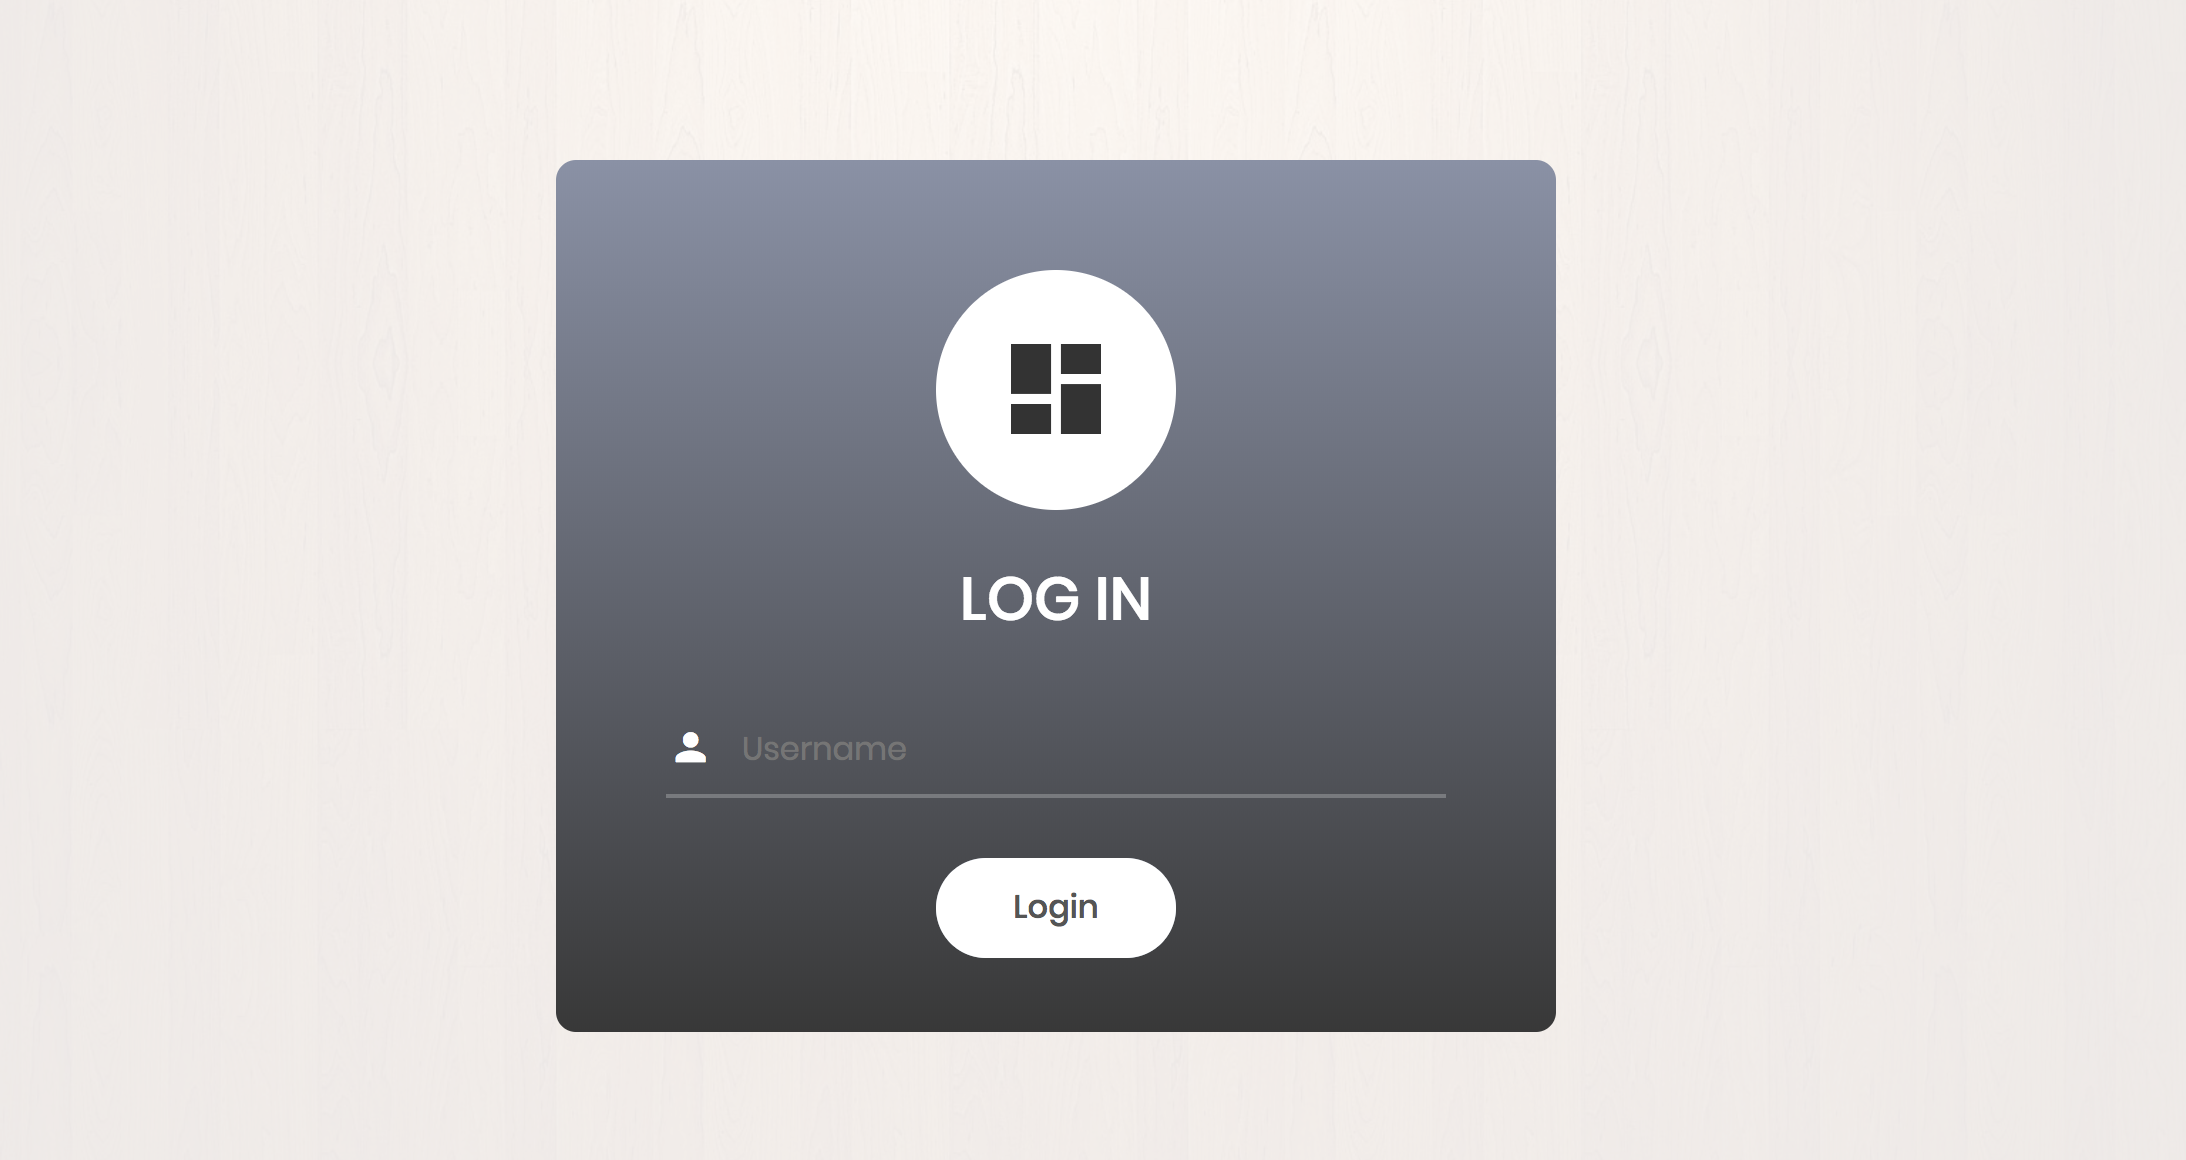
\includegraphics[height=2.0in, width=3.3in]{login.png}
\caption{\texttt{Log in Page}}
\end{figure}

\subsection{Lobby Page}
The information shown on the lobby page including game name, game status(user
is waiting for a match/the players currently playing), number of speculators,
and a column indicates choice of joining or speculating one game. Notice that 
when the lobby is empty, the user receive empty lobby alert instead of being
directed to empty lobby.
\begin{figure}[!htb]
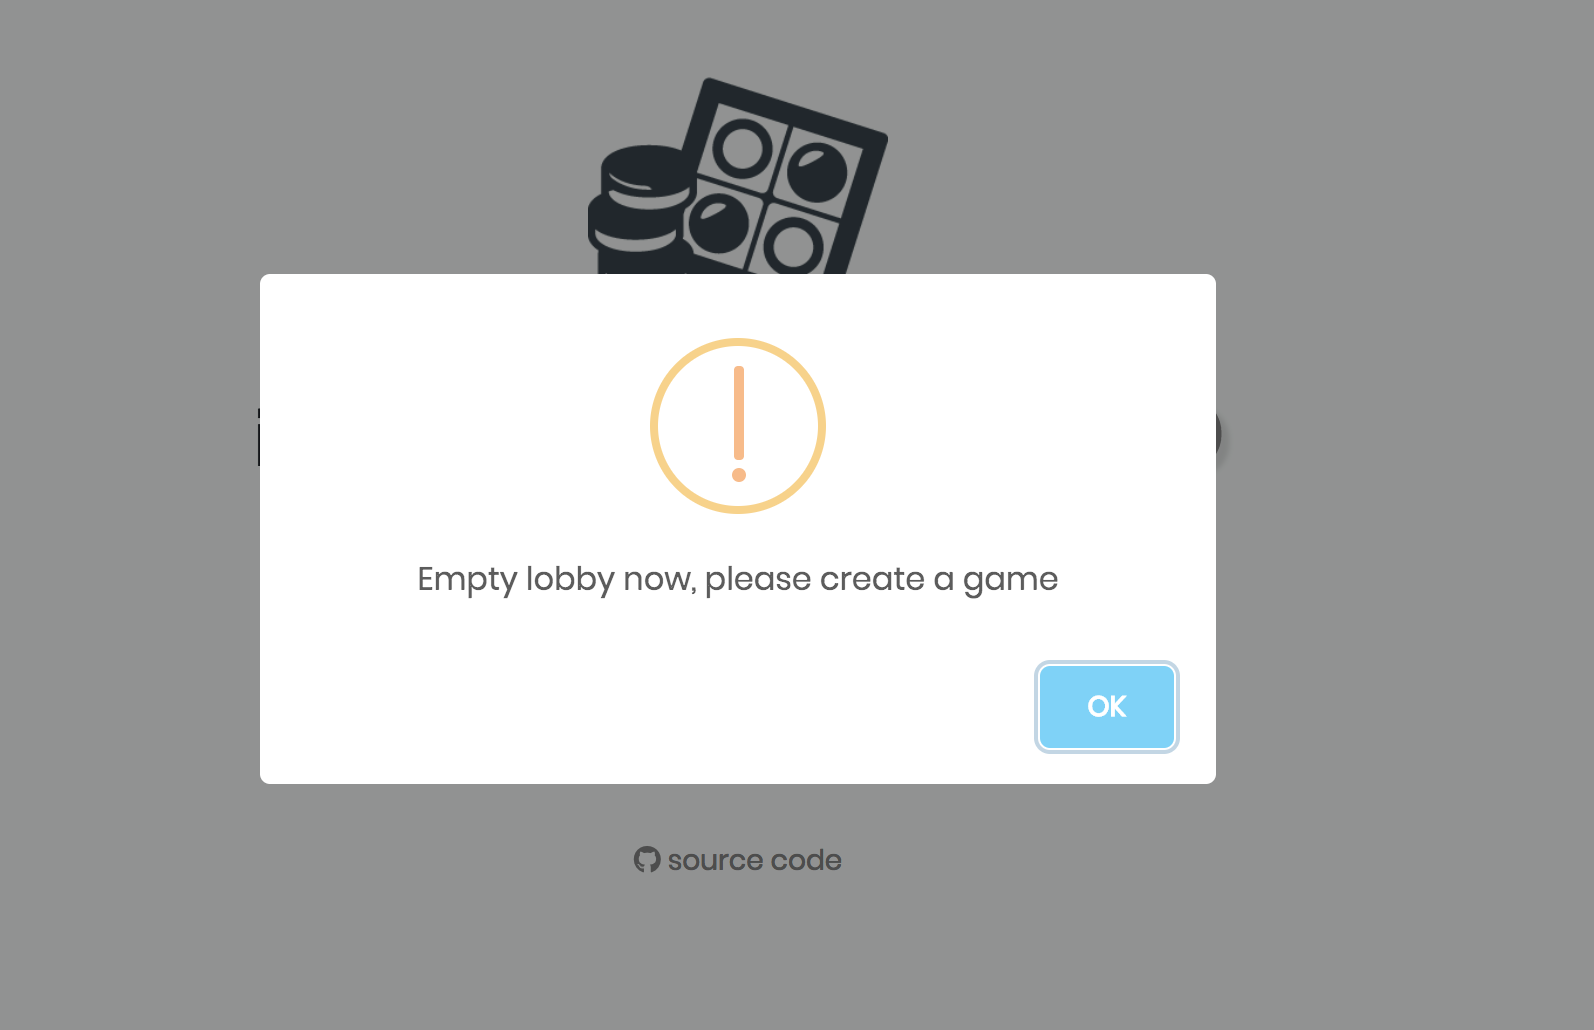
\includegraphics[height=2.0in, width=3.3in]{lobby.png}
\caption{\texttt{Empty Lobby}}
\end{figure}
\begin{figure}[!htb]
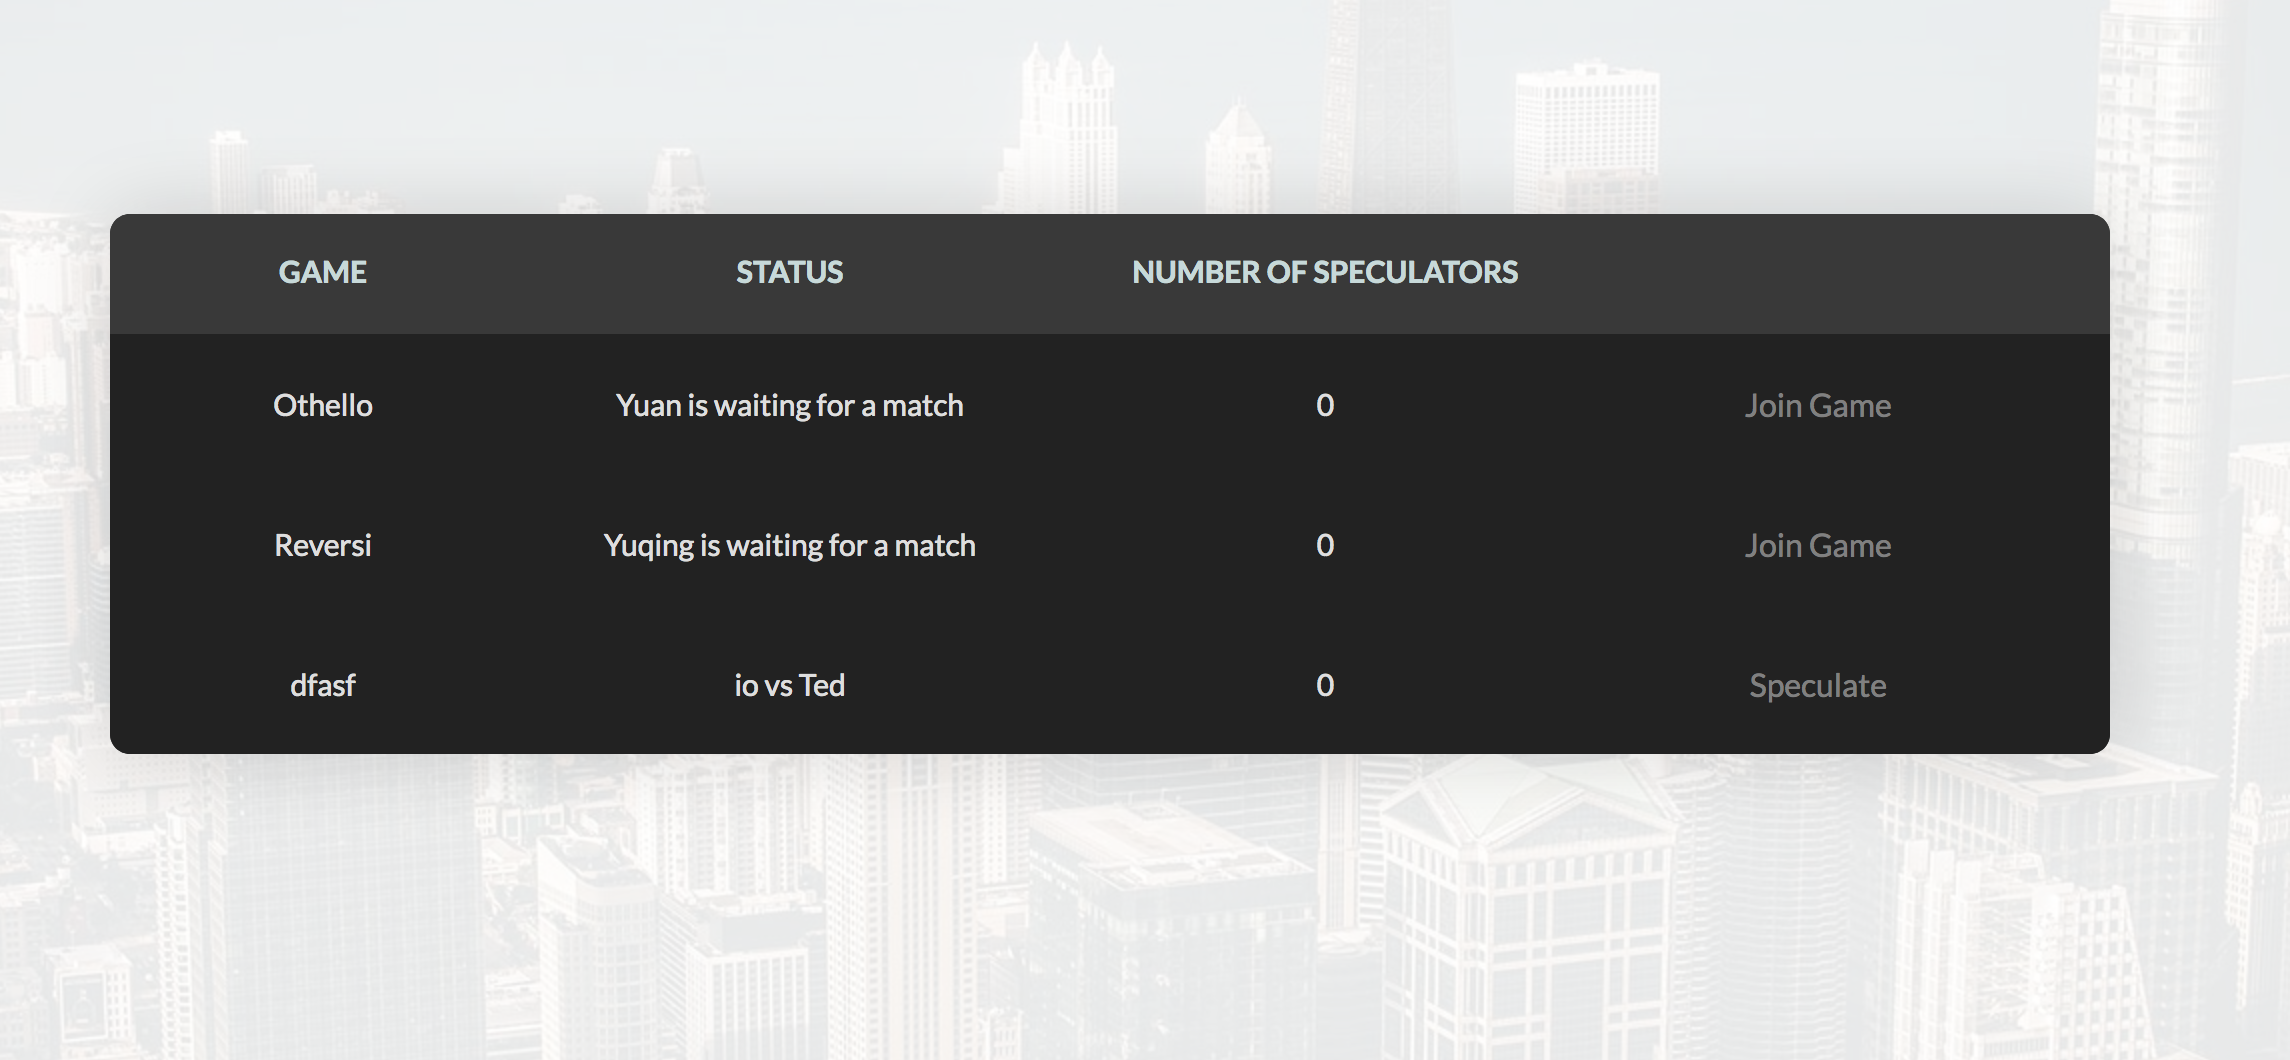
\includegraphics[height=2.0in, width=3.3in]{lobby2.png}
\caption{\texttt{Lobby Page}}
\end{figure}

\subsection{Game Page}
In the game page, there are three main sections.
\begin{itemize}
  \item Header shows the game info, including game name, and game status(waiting
  for a match or players name who are currently playing).
  \item Side bar shows all the speculators' names and has one exit button for 
  a player to exit a game.
  \item Game board uses react-konva component. The disc uses Circle, the board 
  uses Rect, and board line uses Line. On right side of board shows the ownership
  of current move, and number of white and black discs.

\end{itemize}
\begin{figure}[!htb]
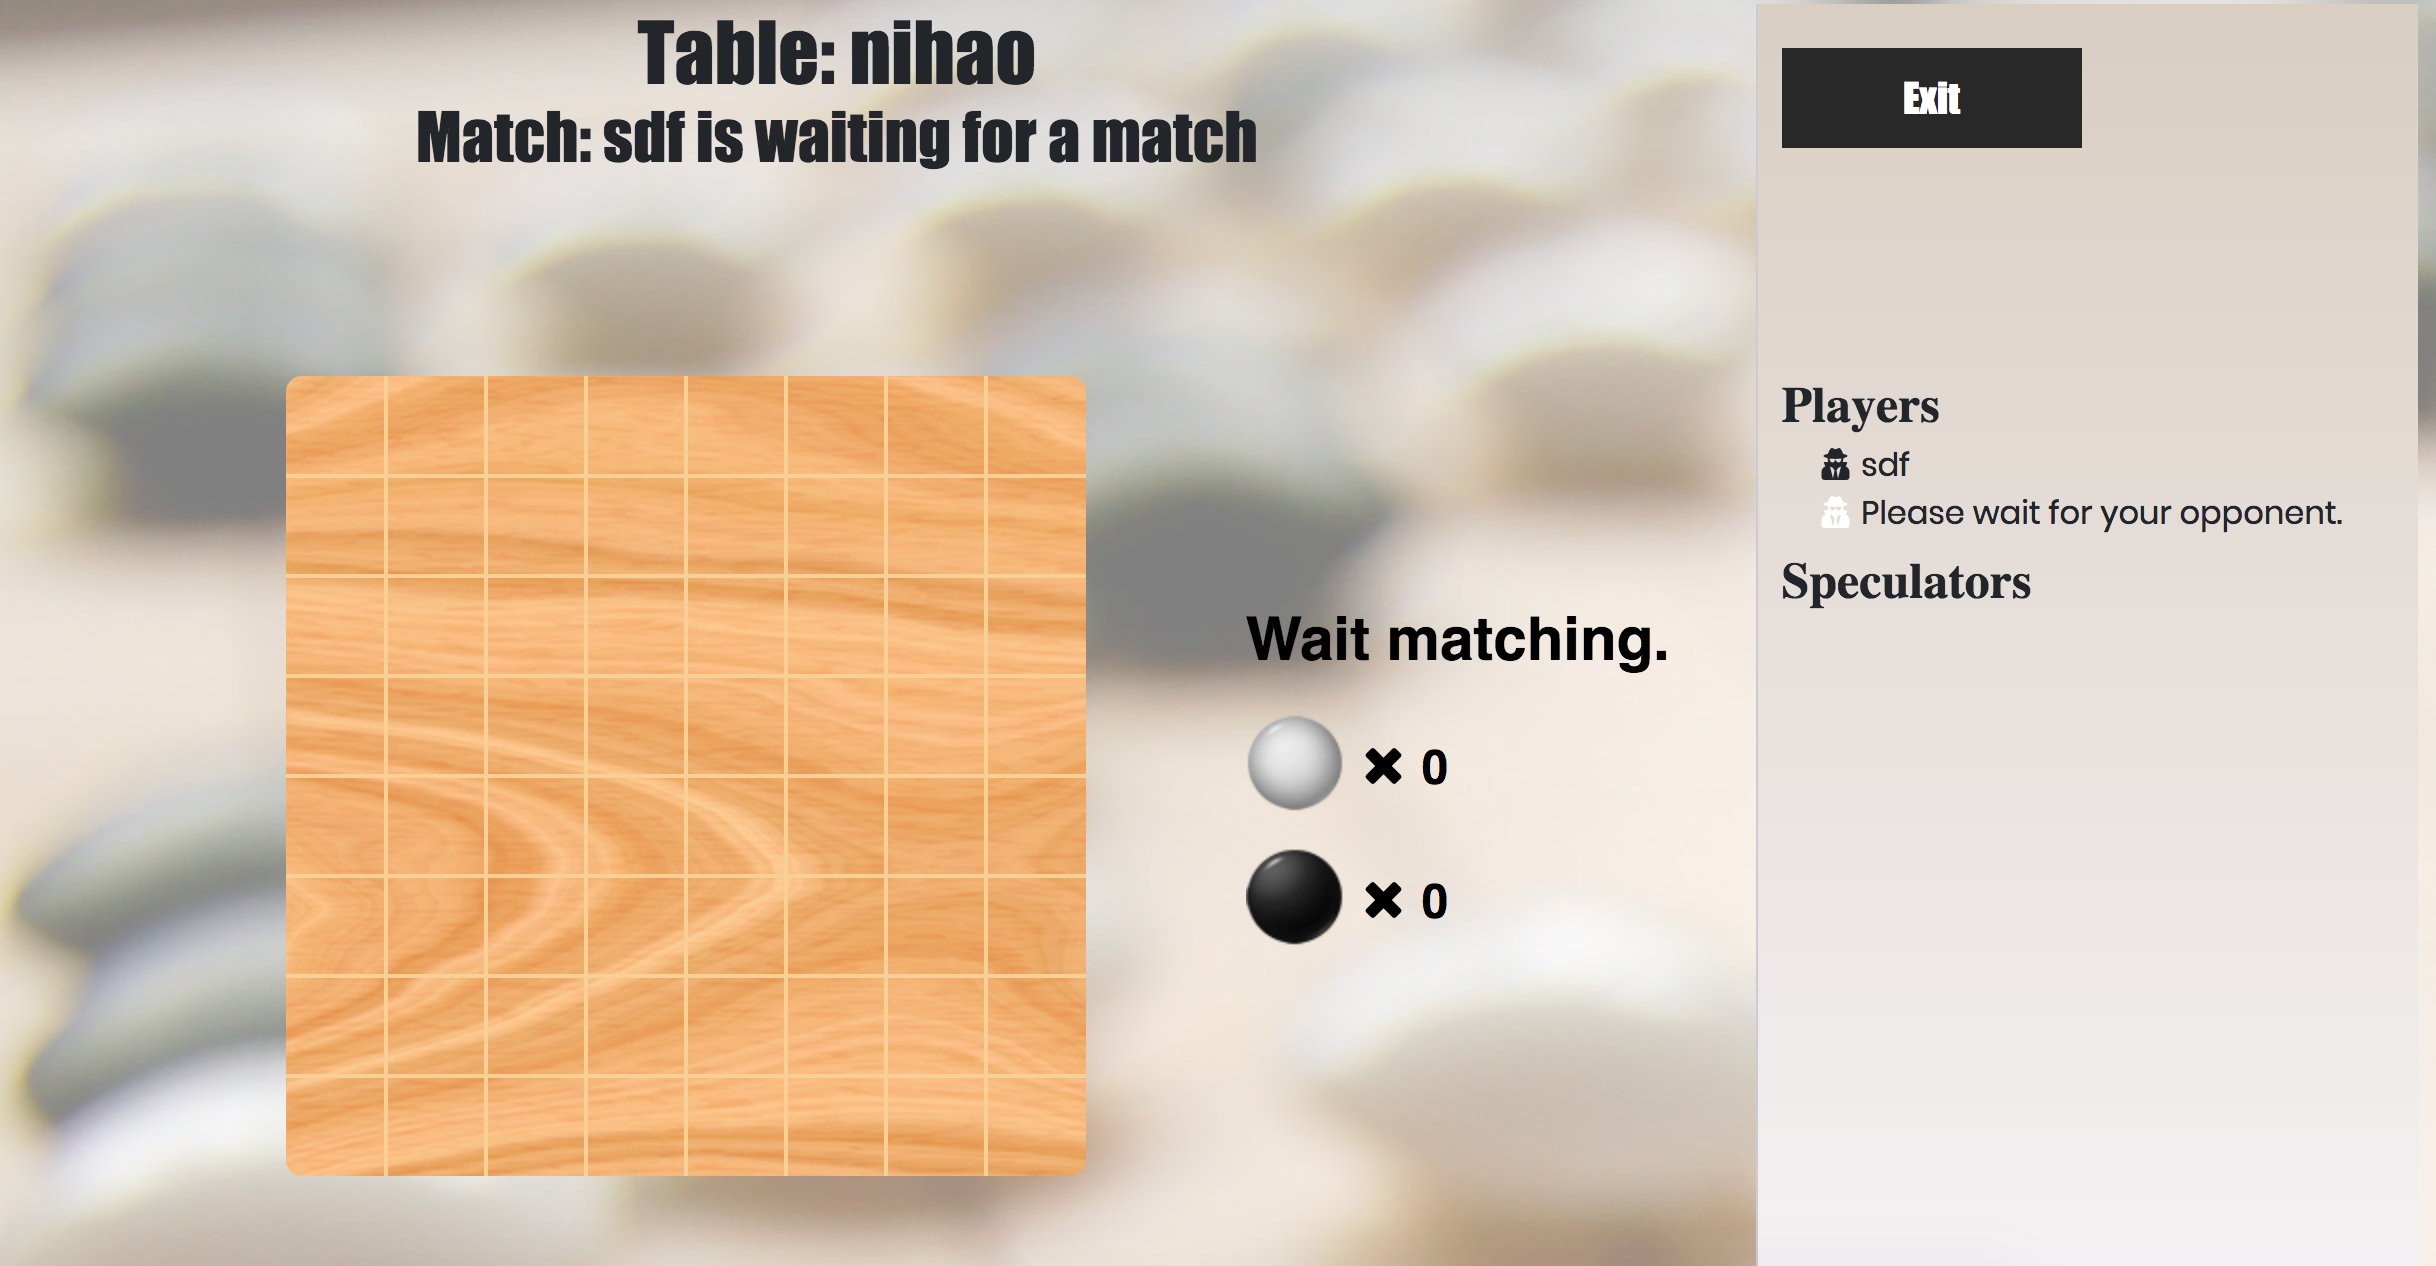
\includegraphics[height=2.0in, width=3.3in]{game.png}
\caption{\texttt{Game Page}}
\end{figure}
\section{UI to Server Protocal}
In this project, there are two types of connection from UI to Server. For page 
rendering and user login, the connection is supported by Phoenix controllers 
invoked from the router in response to HTTP requests (as used in Tasktracker 
homework). For game joining, game state update and broadcasting, the connection 
is supported by websocket implemented by Phoenix channel, which provides a 
bidirectional communication from UI to server.

\subsection{HTTP request and Controllers}
The paths under router.ex are shown as following:

\begin{lstlisting}
get "/", PageController, :index
get "/login", PageController, :login
get "/lobby", PageController, :lobby
get "/game/:game", PageController, :game

post "/session", SessionController, :create
delete "/session", SessionController, :delete
\end{lstlisting}

PageController handles all page requests, and SessionController only handles 
login/logout operations. PageController is invoked as corresponding function 
calls by Router, and corresponding templates are rendered. 

SessionController is invoked in login template and uses put\_session to assign 
username to window session. In router.ex, we also added a plug :get\_current\_user, 
by which the username can be retrieved from session in any template. Based on 
this, we can use <script> in game template to assign session username to window, 
by which a socket can obtain session username for later use in channel.


\subsection{Websocket and Channel}
In user\_socket.ex, we defined channel as "gamechannel:*", where the "*" stands 
for specific name of game table. Therefore a instance of channel stands for a 
specific game table. 

 When a user joins a game (no matter as a player or a speculator), the user just 
 provides the channel name that stands for the name of game table, as well as 
 the socket that contains username originally from session. The join function 
 in game\_channel.ex will invoke module in game.ex to handle the real joining 
 logic, e.g. whether the game exists or needs to be created in Agent, or 
 whether the user joined as a player or speculator...

 We will cover in more details about the data structure on server in later part 
 of the report, but to illustrate the payload structure, we just put our 
 server-side data structure here:

 \begin{lstlisting}
 %{ 
  colors: [],          # a list of numbers of length 64
  turn: 0,             # a number to indicate who's turn, the 
                         number is the index in players
  players: [],         # a list of string that stands for 
                         players
  winner: nil,         # a number that stands for the winner, 
                         nil if no winner
  speculators: [],     # a list of string that stands for 
                         speculators
  online_players: 2    # number of players remained online in 
                         this table
  }
  \end{lstlisting}

  The above data structure stands for a state of game in a game table, 
  which has uniform structure through UI to Server, and we will call it "state" 
  or "game state" in later parts for simplicity. After a join function is called, 
  it wraps and returns a response through socket in a structure like this: 
\begin{lstlisting}
%{"state" => state, "msg" => "message to be displayed", "type" => "optional type"}
\end{lstlisting}

where state is the current game state, which has a structure we discussed above. 
The "msg" stands for the message to be displayed at front-end to notify a new 
user/speculator has joined/left. "type" stands for what kind of notification or 
dialog(success, warning or error) should be displayed.

Apart from a direct return, the join function also triggers handle\_info
({:after\_join, resp}, socket) to be invoked after joining, where resp is 
identical with the reponse passed to socket. In this handle\_info function, 
we broadcast resp to every socket that subsribed to this channel 
(this game table). In this way, every player and speculator will be notified 
that a new player or new speculator has joined this room/table, or a player 
comes back to this room/table. This broadcast has a label "new:user", and the 
callback in front-end's channel.on("new:user") will be called to determine 
how the notification will be executed according to the resp["msg"] and \\
resp["type"].

When a player clicks a position on game board, the UI pushes "move" through 
the socket to server by channel.push("move", {index: index}), where index is 
the index in the 1-D array of colors calculated by x and y coordinates. 
Therefore, the index in 1-D array is the only variable passed to server 
in order to make a move. In game\_channel.ex, handle\_in("move", \%{"index" => i}, 
socket) will be invoked and passed i to Game.simulate\_next\_state(curr\_name, i) 
in game.ex, curr\_name is the current table name that can be retrieved from socket.
The Game.simulate\_next\_state/2 function returns a tuple {boolean, resp}, 
where the boolean indicates whether this move is a valid move, and resp has a 
structure like this:
 \begin{lstlisting}
%{"state" => state}
 \end{lstlisting}

where state is the current game state. If current move is a valid move, 
resp will be broadcasted to every socket subscribed, and {:ok, resp} will 
be returned. If move is invalid, resp will not be broadcasted, and {:error, 
resp} will be returned. In client-side, if channel detects "error" in call-back, 
the player will be notified that the current move is invalid.

When any user leaves the game table (close browser, log out or go to another 
page), terminate(reason, socket) will be called. The terminate/2 determines 
whether the game table should persist and what kind of message should be 
broadcasted, the broadcasted payload has a structure like this:

 \begin{lstlisting}
 %{"msg" => msg, "type" => type}
\end{lstlisting}


\section{Data structures on server}
As discussed before, the game state on server has a structure like this:
\begin{lstlisting}
%{ 
  colors: [],        # a list of numbers of length 64
  turn: 0 or 1,      # a number to indicate who's turn, the 
                       number is the index in players
  players: [],       # a list of string that stands for 
                       players
  winner: nil,       # a number that stands for the winner, 
                       nil if no winner
  speculators: [],   # a list of string that stands for 
                       speculators
  online_players: 2  # number of players remained online in 
                       this table
  }
\end{lstlisting}
More specifically, each element in the color list stands for the occupation or 
color on this position, 0 represents unoccupied, 1 represents black disc, and 
2 represents white disc. The list of players and list of speculators are both 
lists of usernames. The "turn" attribute is the index in players, the username 
of owner of this turn is players[turn]. The "winner" attribute uses the similar 
design, players[winner] is the username of the winner, but apart from 0 and 1, 
"winner" attribute can also be 2, which stands for a tie situation when game 
ends. The online\_players stands for the number of online players remained in 
this table, when online\_players becomes 0, the game table will be closed and 
deleted as introduced in our design part.

Game states all persist on Agent in server. The Agent in our project has a 
structure like this:
\begin{lstlisting}
%Agent{games: %{game_name: state}}
\end{lstlisting}
Under this design, Agent.get(:games, \&(\&1)) will get all game states in a form 
of map, and this map can get a specific game state using the game\_name as key. 
The reason why we chose not to directy use {game\_name => state} as key-value 
pair under Agent is that, in order to implement game lobby, we want the whole 
list of game states, and Agent.get(:games, \&(\&1)) can simply achieve this. The 
trade-off is, this makes us need to get all game states before retrieving a 
specific state, and each game state has O(n) complexity, where n is number of 
users (players and speculators list), if there are m rooms, the space complexity 
can be O(mn). However, as this is a course project, even if we have 1000 users 
and 1000 rooms, the worst-case memory used is just O(1000,000), which can 
actually use only MBs of memory, therefore making our design totally acceptable.

\section{Implementation of game rules}
All game rules are implemented under a single module in game.ex. Apart from game rules, game.ex also handles how game state would change, whether a user should be a player or a speculator in a joining or leaving game event, as well as winner check. In general, it handles all behind-the-scene app logic/intelligence, which is the "model" portion of a MVC pattern.

As for game rules, imagine we have a game board, each time a player clicks a position on this board, the algorithm would check in 8 directions (up, down, left, right, up-left, up-right, down-left, down-right) from this position to determine whether there exists a disc in the same color so that all opponent's discs along the path could flip. Since Elixir is a functional language, we implemented the above algorithm using recursion in the function check_swaps/4. Besides check_swaps/4, there is in_bound/2 function working with it to make sure not going out of bound. Also, valid_next/2 function is used to filter the cases when the next adjacent disc is in the same color, i.e. a valid move should flip at least one opponent's disc.

It's worth noticing that in Othello, in some cases, in one player's turn, the player cannot find any valid move in order to flip opponent's discs. According to many examples of Othello games, they handle this problem by simply giving the current turn to this player's opponent, and we adopted this game rule in our design. Futhermore, even if the opponent take over the turn, the opponent might also not have a valid move, in this case, as both players don't have a valid move, we will start counting number of discs to produce and announce a winner. In our algorithm, a valid next move check will be done after one player successfully makes a move. In the valid next move check, every spare place on board is checked to determine whether the opponent can make a valid move here, if no such place exists, the turn of game state will remain the same and this will be notified at front-end. If current player cannot move, either, a winner will be determined and announced. The time complexity of this process might sound high, i.e. if total positions on board is N, our algorithm is approximately O(N^2), but there are totally only 64 positions on board, that is, the input size of our algorithm is very small in nature, so the server would definitely afford an "inefficient" algorithm, not to mention it's still poly-nomial.

Check winner is also an important part of game rules. In most cases, players fill up all spaces on board, and player with more discs on the board becomes winner. Besides, as discussed above, if both players cannot make a valid move, the player with more disc on the board becomes winner. Moreover, a special case of the second case is that when all colors of discs on board become identical, this should be combined in second case. These logics are implemented with get_num_colors/3 function to count the number of discs in each color. Similar to check_swaps/4, get_num_colors/3 is also implemented using recursion.


\section{Challenges and Solutions}




\begin{comment}

\begin{acks}
\end{acks}

\subsection{Type Changes and {\itshape Special} Characters}

We have already seen several typeface changes in this sample.  You can
indicate italicized words or phrases in your text with the command
\texttt{{\char'134}textit}; emboldening with the command
\texttt{{\char'134}textbf} and typewriter-style (for instance, for
computer code) with \texttt{{\char'134}texttt}.  But remember, you do
not have to indicate typestyle changes when such changes are part of
the \textit{structural} elements of your article; for instance, the
heading of this subsection will be in a sans serif\footnote{Another
  footnote here.  Let's make this a rather long one to see how it
  looks.} typeface, but that is handled by the document class file.
Take care with the use of\footnote{Another footnote.}  the
curly braces in typeface changes; they mark the beginning and end of
the text that is to be in the different typeface.

You can use whatever symbols, accented characters, or non-English
characters you need anywhere in your document; you can find a complete
list of what is available in the \textit{\LaTeX\ User's Guide}
\cite{Lamport:LaTeX}.

\subsection{Math Equations}
You may want to display math equations in three distinct styles:
inline, numbered or non-numbered display.  Each of
the three are discussed in the next sections.

\subsubsection{Inline (In-text) Equations}
A formula that appears in the running text is called an
inline or in-text formula.  It is produced by the
\textbf{math} environment, which can be
invoked with the usual \texttt{{\char'134}begin\,\ldots{\char'134}end}
construction or with the short form \texttt{\$\,\ldots\$}. You
can use any of the symbols and structures,
from $\alpha$ to $\omega$, available in
\LaTeX~\cite{Lamport:LaTeX}; this section will simply show a
few examples of in-text equations in context. Notice how
this equation:
\begin{math}
  \lim_{n\rightarrow \infty}x=0
\end{math},
set here in in-line math style, looks slightly different when
set in display style.  (See next section).

\subsubsection{Display Equations}
A numbered display equation---one set off by vertical space from the
text and centered horizontally---is produced by the \textbf{equation}
environment. An unnumbered display equation is produced by the
\textbf{displaymath} environment.

Again, in either environment, you can use any of the symbols
and structures available in \LaTeX\@; this section will just
give a couple of examples of display equations in context.
First, consider the equation, shown as an inline equation above:
\begin{equation}
  \lim_{n\rightarrow \infty}x=0
\end{equation}
Notice how it is formatted somewhat differently in
the \textbf{displaymath}
environment.  Now, we'll enter an unnumbered equation:
\begin{displaymath}
  \sum_{i=0}^{\infty} x + 1
\end{displaymath}
and follow it with another numbered equation:
\begin{equation}
  \sum_{i=0}^{\infty}x_i=\int_{0}^{\pi+2} f
\end{equation}
just to demonstrate \LaTeX's able handling of numbering.

\subsection{Citations}
Citations to articles~\cite{bowman:reasoning,
clark:pct, braams:babel, herlihy:methodology},
conference proceedings~\cite{clark:pct} or maybe
books \cite{Lamport:LaTeX, salas:calculus} listed
in the Bibliography section of your
article will occur throughout the text of your article.
You should use BibTeX to automatically produce this bibliography;
you simply need to insert one of several citation commands with
a key of the item cited in the proper location in
the \texttt{.tex} file~\cite{Lamport:LaTeX}.
The key is a short reference you invent to uniquely
identify each work; in this sample document, the key is
the first author's surname and a
word from the title.  This identifying key is included
with each item in the \texttt{.bib} file for your article.

The details of the construction of the \texttt{.bib} file
are beyond the scope of this sample document, but more
information can be found in the \textit{Author's Guide},
and exhaustive details in the \textit{\LaTeX\ User's
Guide} by Lamport~\shortcite{Lamport:LaTeX}.

This article shows only the plainest form
of the citation command, using \texttt{{\char'134}cite}.

Some examples.  A paginated journal article \cite{Abril07}, an enumerated
journal article \cite{Cohen07}, a reference to an entire issue \cite{JCohen96},
a monograph (whole book) \cite{Kosiur01}, a monograph/whole book in a series (see 2a in spec. document)
\cite{Harel79}, a divisible-book such as an anthology or compilation \cite{Editor00}
followed by the same example, however we only output the series if the volume number is given
\cite{Editor00a} (so Editor00a's series should NOT be present since it has no vol. no.),
a chapter in a divisible book \cite{Spector90}, a chapter in a divisible book
in a series \cite{Douglass98}, a multi-volume work as book \cite{Knuth97},
an article in a proceedings (of a conference, symposium, workshop for example)
(paginated proceedings article) \cite{Andler79}, a proceedings article
with all possible elements \cite{Smith10}, an example of an enumerated
proceedings article \cite{VanGundy07},
an informally published work \cite{Harel78}, a doctoral dissertation \cite{Clarkson85},
a master's thesis: \cite{anisi03}, an online document / world wide web
resource \cite{Thrun02d}, a video game (Case 1) \cite{Wikipedia} and (Case 2) \cite{CS188}



\subsection{Tables}
Because tables cannot be split across pages, the best
placement for them is typically the top of the page
nearest their initial cite.  To
ensure this proper ``floating'' placement of tables, use the
environment \textbf{table} to enclose the table's contents and
the table caption.  The contents of the table itself must go
in the \textbf{tabular} environment, to
be aligned properly in rows and columns, with the desired
horizontal and vertical rules.  Again, detailed instructions
on \textbf{tabular} material
are found in the \textit{\LaTeX\ User's Guide}.

Immediately following this sentence is the point at which
Table~\ref{tab:freq} is included in the input file; compare the
placement of the table here with the table in the printed
output of this document.

\begin{table}
  \caption{Frequency of Special Characters}
  \label{tab:freq}
  \begin{tabular}{ccl}
    \toprule
    Non-English or Math&Frequency&Comments\\
    \midrule
    \O & 1 in 1,000& For Swedish names\\
    $\pi$ & 1 in 5& Common in math\\
    \$ & 4 in 5 & Used in business\\
    $\Psi^2_1$ & 1 in 40,000& Unexplained usage\\
  \bottomrule
\end{tabular}
\end{table}

To set a wider table, which takes up the whole width of the page's
live area, use the environment \textbf{table*} to enclose the table's
contents and the table caption.  As with a single-column table, this
wide table will ``float'' to a location deemed more desirable.
Immediately following this sentence is the point at which
Table~\ref{tab:commands} is included in the input file; again, it is
instructive to compare the placement of the table here with the table
in the printed output of this document.


\begin{table*}
  \caption{Some Typical Commands}
  \label{tab:commands}
  \begin{tabular}{ccl}
    \toprule
    Command &A Number & Comments\\
    \midrule
    \texttt{{\char'134}author} & 100& Author \\
    \texttt{{\char'134}table}& 300 & For tables\\
    \texttt{{\char'134}table*}& 400& For wider tables\\
    \bottomrule
  \end{tabular}
\end{table*}
% end the environment with {table*}, NOTE not {table}!



\subsection{Figures}

Like tables, figures cannot be split across pages; the best placement
for them is typically the top or the bottom of the page nearest their
initial cite.  To ensure this proper ``floating'' placement of
figures, use the environment \textbf{figure} to enclose the figure and
its caption.

This sample document contains examples of \texttt{.eps} files to be
displayable with \LaTeX.  If you work with pdf\LaTeX, use files in the
\texttt{.pdf} format.  Note that most modern \TeX\ systems will convert
\texttt{.eps} to \texttt{.pdf} for you on the fly.  More details on
each of these are found in the \textit{Author's Guide}.

\begin{figure}
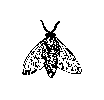
\includegraphics{fly}
\caption{A sample black and white graphic.}
\end{figure}

\begin{figure}
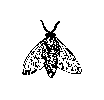
\includegraphics[height=1in, width=1in]{fly}
\caption{A sample black and white graphic
that has been resized with the \texttt{includegraphics} command.}
\end{figure}




\begin{figure*}
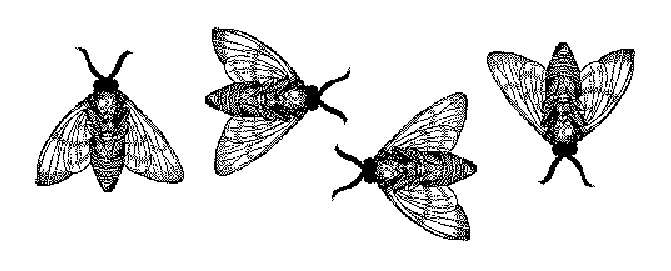
\includegraphics{flies}
\caption{A sample black and white graphic
that needs to span two columns of text.}
\end{figure*}


\begin{figure}
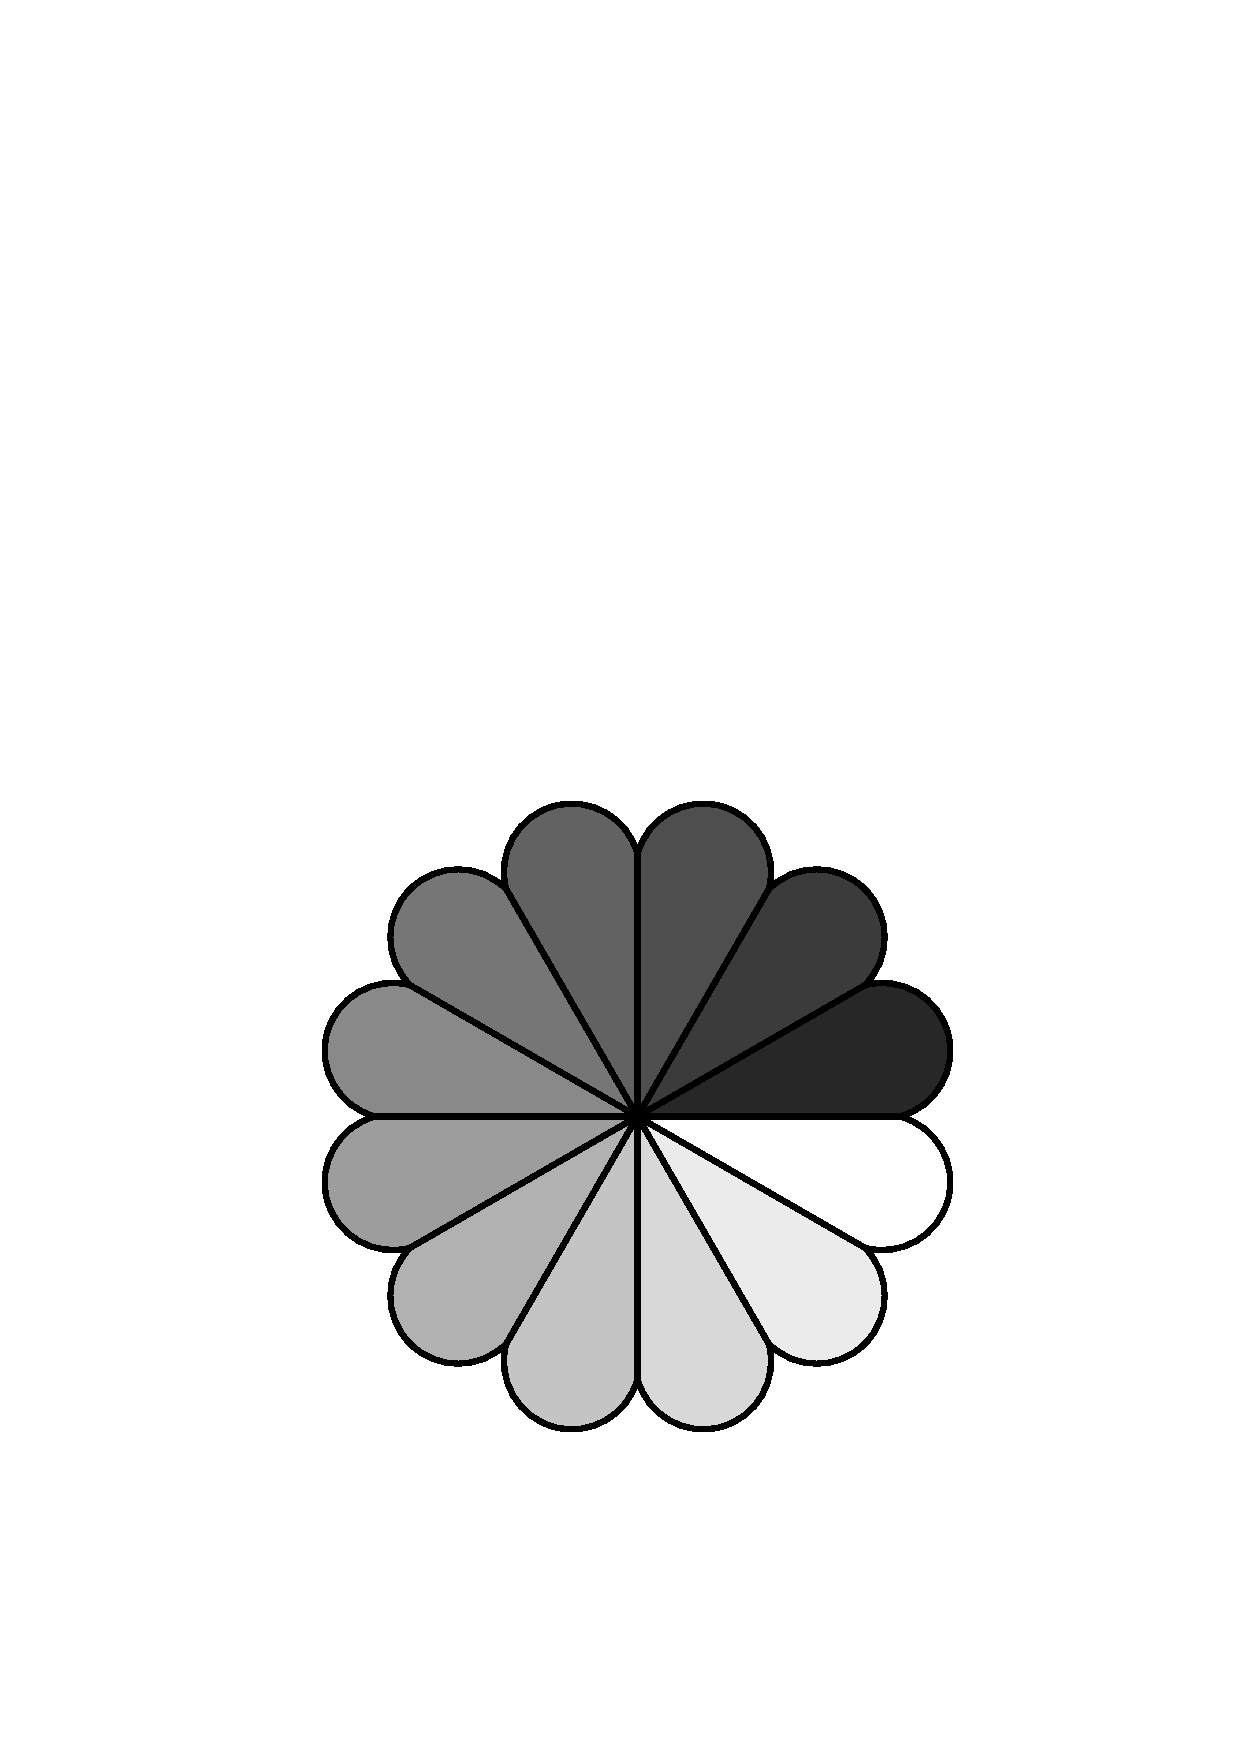
\includegraphics[height=1in, width=1in]{rosette}
\caption{A sample black and white graphic that has
been resized with the \texttt{includegraphics} command.}
\end{figure}


%\end{document}  % This is where a 'short' article might terminate



\appendix
%Appendix A
\section{Headings in Appendices}
The rules about hierarchical headings discussed above for
the body of the article are different in the appendices.
In the \textbf{appendix} environment, the command
\textbf{section} is used to
indicate the start of each Appendix, with alphabetic order
designation (i.e., the first is A, the second B, etc.) and
a title (if you include one).  So, if you need
hierarchical structure
\textit{within} an Appendix, start with \textbf{subsection} as the
highest level. Here is an outline of the body of this
document in Appendix-appropriate form:
\subsection{Introduction}
\subsection{The Body of the Paper}
\subsubsection{Type Changes and  Special Characters}
\subsubsection{Math Equations}
\paragraph{Inline (In-text) Equations}
\paragraph{Display Equations}
\subsubsection{Citations}
\subsubsection{Tables}
\subsubsection{Figures}
\subsubsection{Theorem-like Constructs}
\subsubsection*{A Caveat for the \TeX\ Expert}
\subsection{Conclusions}
\subsection{References}
Generated by bibtex from your \texttt{.bib} file.  Run latex,
then bibtex, then latex twice (to resolve references)
to create the \texttt{.bbl} file.  Insert that \texttt{.bbl}
file into the \texttt{.tex} source file and comment out
the command \texttt{{\char'134}thebibliography}.
% This next section command marks the start of
% Appendix B, and does not continue the present hierarchy
\section{More Help for the Hardy}

Of course, reading the source code is always useful.  The file
\path{acmart.pdf} contains both the user guide and the commented
code.
\end{comment}

